%=========================================================================
% Start of
%=========================================================================
\preClass{Linear Functions}

\begin{problem}
\item A tortoise and a hare move in a straight line, and the both
  start at $x=0$. The tortoise's position is given by
  \begin{eqnarray*}
    x_T & = & \frac{1}{2} t,
  \end{eqnarray*}
  where $t$ is in minutes and $x$ is in meters.  The hare's position
  is given by
  \begin{eqnarray*}
    x_H & = & 2 t,
  \end{eqnarray*}
  where $t$ is in minutes and $x$ is in meters.
  \begin{subproblem}
  \item Determine the positions of the tortoise at $t=0$, $t=1$, and
    $t=2$.
    \vfill
  \item Determine the positions of the hare at $t=0$, $t=1$, and
    $t=2$.
    \vfill

    \clearpage
  \item For each time, plot the coordinate of the relative positions
    on the set of axes below. Use the tortoise's position for the
    $x$-coordinate, and use the hare's position for the
    $y$-coordinate. For example, if the tortoise's position is 1m, and
    the hare's position is 4m, then the coordinate would be $P(1,4)$.

    \begin{tikzpicture}[y=1.1cm, x=1.1cm,font=\sffamily]
        % bounds
        \def\lowX{-5.5}
        \pgfmathtruncatemacro\startX{round(0.5+\lowX)}
        \pgfmathsetmacro\nextXValue{int(\startX+1)}
        \def\highX{5.5}
        \def\lowY{-5.5}
        \def\highY{5.5}
        \pgfmathsetmacro\nextYValue{int(\lowY+1)}
        % ticks
        \draw[step = 1, gray, very thin,dashed,opacity=0.85] (\lowX, \lowY) grid ( \highX,\highY);
     	% axis
    	\draw[thick,->] (\lowX,0) -- coordinate (x axis mid) (\highX,0)
                  node[anchor = south] {Hare's Position (m)};
        \draw[thick,->] (0,\lowY) -- coordinate (y axis mid) (0,\highY)
                  node[anchor = south east] {Tortoise's Position (m)};
        \foreach \y in {-5,-4,...,-1,1,2,...,\highY} {
          \draw (1pt, \y) -- (-1pt, \y) node[yshift=-6,xshift=-1,anchor=east] {$\y$};
        }
        \foreach \x in {-5,-4,...,-1,1,2,...,\highX} {
          \draw (\x,1pt) -- (\x,-1pt) node[yshift=-5,xshift=0,anchor=east] {$\x$};
        }
        \draw (0,6.0) node [anchor=south] {Hare vs. Tortoise};
      \end{tikzpicture}

  \end{subproblem}

\clearpage

\item A tortoise and a hare move in a straight line, and the both
  start at $x=0$. The tortoise's position is given by
  \begin{eqnarray}
    \label{actLinear:eqn:tortoise}
    x_T & = & \frac{1}{2} t,
  \end{eqnarray}
  where $t$ is in minutes and $x$ is in meters.  The hare's position
  is given by
  \begin{eqnarray}
    \label{actLinear:eqn:hare}
    x_H & = & 2 t,
  \end{eqnarray}
  where $t$ is in minutes and $x$ is in meters.

  Determine the relationship between the hare's and the tortoise's
  position. That is, given the hare's position determine the
  tortoise's position. Make a sketch of the graph of the relationship using the axes below.

  \begin{tikzpicture}[y=1.1cm, x=1.1cm,font=\sffamily]
      % bounds
      \def\lowX{-5.5}
      \pgfmathtruncatemacro\startX{round(0.5+\lowX)}
      \pgfmathsetmacro\nextXValue{int(\startX+1)}
      \def\highX{5.5}
      \def\lowY{-5.5}
      \def\highY{5.5}
      \pgfmathsetmacro\nextYValue{int(\lowY+1)}
      % ticks
      \draw[step = 1, gray, very thin,dashed,opacity=0.85] (\lowX, \lowY) grid ( \highX,\highY);
    % axis
    	\draw[thick,->] (\lowX,0) -- coordinate (x axis mid) (\highX,0)
                  node[anchor = south] {Hare's Position (m)};
        \draw[thick,->] (0,\lowY) -- coordinate (y axis mid) (0,\highY)
                  node[anchor = south east] {Tortoise's Position (m)};
      \foreach \y in {-5,-4,...,-1,1,2,...,\highY} {
        \draw (1pt, \y) -- (-1pt, \y) node[yshift=-6,xshift=-1,anchor=east] {$\y$};
      }
      \foreach \x in {-5,-4,...,-1,1,2,...,\highX} {
        \draw (\x,1pt) -- (\x,-1pt) node[yshift=-5,xshift=-1,anchor=east] {$\x$};
      }
      \draw (0,6) node [anchor=south] {Hare vs. Tortoise};
    \end{tikzpicture}


    What is the tortoise's position when the hare's position is 15
    meters? (Mark the associated coordinate on the plot above.)

    In equation \ref{actLinear:eqn:tortoise} and
    \ref{actLinear:eqn:hare} how many variables are there? How many
    equations? Which variables are changing?

\end{problem}


\actTitle{Linear Equations}
\begin{problem}
\item In each case below determine the formulas for the lines that
  satisfy the given requirements. In each case make a rough sketch of
  the line.

  \begin{subproblem}
  \item Goes through the point $P(-2,5)$ and has a slope of -3.
    \vfill
  \item Goes through the points $P_1(-3,-4)$ and $P_2(4,1)$.
    \vfill
  \end{subproblem}

  \clearpage

\item Two test plots are used to study the spread of an invasive
  plant. In the first test plot the conditions are dryer than in the
  second test plot. In the first test plot the invasive plant begins
  with a coverage of 10 square meters, and each day the area covered
  by the plant increases by 2 square meters. In the second test plot
  the invasive plant begins with a coverage of 15 square meters, and
  each day the area increases by 1 square meters.

  \begin{subproblem}
  \item Will there be a time when the area covered by the invasive
    test plant will be the same in the two test plots. Explain your
    reasoning.  
    \vfill

  \item Determine the area covered by the invasive plant in each test
    plot for a given time.
    \vfill

  \item Determine the time that the area covered will be the same.
    \vfill
  \end{subproblem}

  \clearpage

\item A group of researchers studies birds near a park. The birds tend
  to use cigarette butts in their nests, and it is believed to help
  reduce the number of parasitic insects. It is estimated that the
  number of cigarette butts used for nesting materials varies linearly
  with the distance from the nest to a nearby open air theater. A nest
  that is a distance of 30 meters appears to have 10 cigarette butts,
  and a nest that is a distance of 40 meters appears to have 8
  cigarette butts.
  \begin{subproblem}
  \item Determine the relationship that will predict the number of
    cigarette butts in a nest given its distance from the theater.
    Use the relationship to predict the number of cigarette butts in a
    nest 50 meters from the theater. Also, make a sketch of the
    relationship.  \sideNote{Be sure to label your axes and annotate
      your plot.}

    \vfill
    \vfill
    \vfill

  \item What is the domain for the relationship?
    \vfill
  \item A nest is found that has 4 cigarette butts. What is the
    prediction for the distance the nest is from the theater.
    \vfill
  \item If the conjecture for the reason why birds use cigarette butts
    in their nests is true what would you expect is the general
    relationship between the fledgling success rate for birds and the
    location of their nests?
  \end{subproblem}

  \clearpage

\item For the lines in the following plot sort the slopes for the
  lines in increasing order. (Write out the slopes, $m_1$, $m_2$,
  etc., in order from lowest to highest and do not try to estimate
  their values.)

  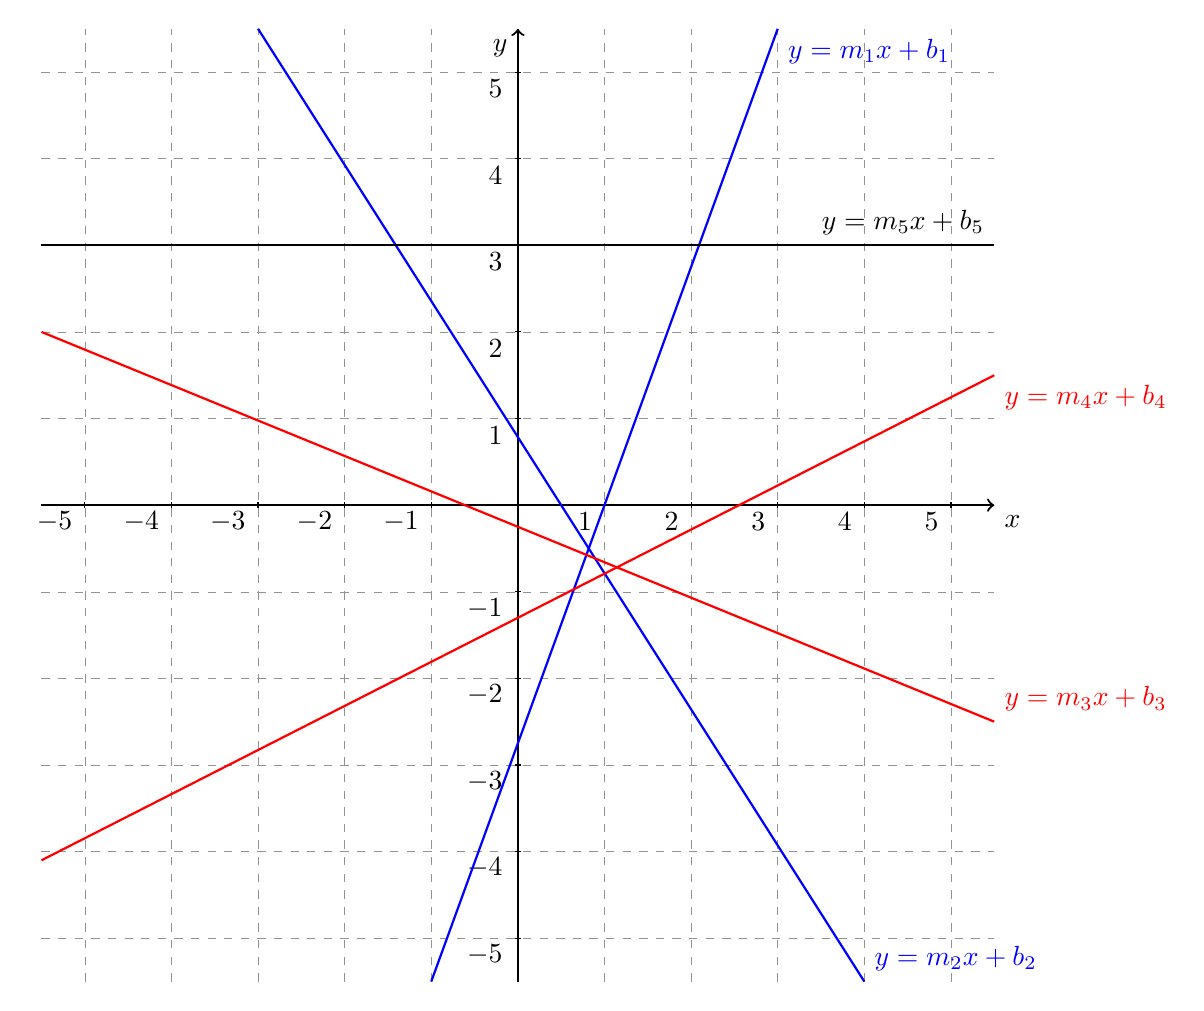
\begin{tikzpicture}[y=1.1cm, x=1.1cm,font=\sffamily]
    % bounds
    \def\lowX{-5.5}
    \pgfmathtruncatemacro\startX{round(0.5+\lowX)}
    \pgfmathsetmacro\nextXValue{int(\startX+1)}
    \def\highX{5.5}
    \def\lowY{-5.5}
    \def\highY{5.5}
    \pgfmathsetmacro\nextYValue{int(\lowY+1)}
    % ticks
    \draw[step = 1, gray, very thin,dashed,opacity=0.85] (\lowX, \lowY) grid ( \highX,\highY);
    % axis
    \draw[thick,->] (\lowX,0) -- coordinate (x axis mid) (\highX,0) node[anchor = north west] {$x$};
    \draw[thick,->] (0,\lowY) -- coordinate (y axis mid) (0,\highY) node[anchor = north east] {$y$};
    \foreach \y in {-5,-4,...,-1,1,2,...,\highY} {
      \draw (1pt, \y) -- (-1pt, \y) node[yshift=-6,xshift=-1,anchor=east] {$\y$};
    }
    \foreach \x in {-5,-4,...,-1,1,2,...,\highX} {
      \draw (\x,1pt) -- (\x,-1pt) node[yshift=-5,xshift=-1,anchor=east] {$\x$};
    }
        
    % Draw some lines and label them.
    \draw[thick, blue] (  -1,-5.5) -- (  3, 5.5) node[anchor=north west] {$y=m_1 x + b_1$};
    \draw[thick, blue] (  -3, 5.5) -- (  4,-5.5) node[anchor=south west] {$y=m_2 x + b_2$};
    \draw[thick,  red] (-5.5,   2) -- (5.5,-2.5) node[anchor=south west] {$y=m_3 x + b_3$};
    \draw[thick,  red] (-5.5,-4.1) -- (5.5, 1.5) node[anchor=north west] {$y=m_4 x + b_4$};
    \draw[thick,black] (-5.5, 3.0) -- (5.5, 3.0) node[anchor=south east] {$y=m_5 x + b_5$};
  \end{tikzpicture}

  \clearpage

\item For each question below the function, Larry($x$), is defined to be
  \begin{eqnarray*}
    \mathrm{Larry}(x) & = & \frac{1}{2} (x-1)^2+2.
  \end{eqnarray*}
  \begin{subproblem}
  \item Make a sketch of Larry.

    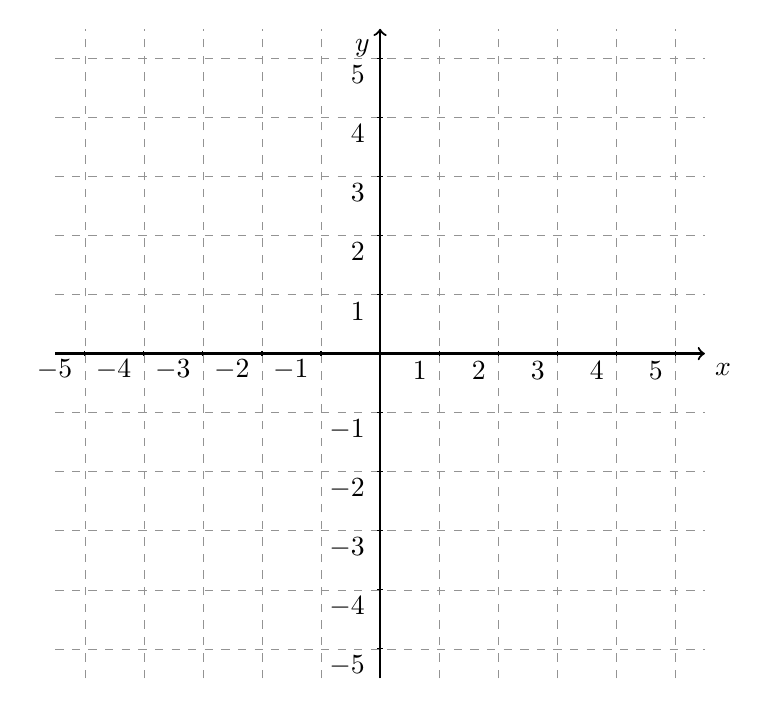
\begin{tikzpicture}[y=0.75cm, x=0.75cm,font=\sffamily]
      % bounds
      \def\lowX{-5.5}
      \pgfmathtruncatemacro\startX{round(0.5+\lowX)}
      \pgfmathsetmacro\nextXValue{int(\startX+1)}
      \def\highX{5.5}
      \def\lowY{-5.5}
      \def\highY{5.5}
      \pgfmathsetmacro\nextYValue{int(\lowY+1)}
      % ticks
      \draw[step = 1, gray, very thin,dashed,opacity=0.85] (\lowX, \lowY) grid ( \highX,\highY);
      % axis
      \draw[thick,->] (\lowX,0) -- coordinate (x axis mid) (\highX,0) node[anchor = north west] {$x$};
      \draw[thick,->] (0,\lowY) -- coordinate (y axis mid) (0,\highY) node[anchor = north east] {$y$};
      \foreach \y in {-5,-4,...,-1,1,2,...,\highY} {
        \draw (1pt, \y) -- (-1pt, \y) node[yshift=-6,xshift=-1,anchor=east] {$\y$};
      }
      \foreach \x in {-5,-4,...,-1,1,2,...,\highX} {
        \draw (\x,1pt) -- (\x,-1pt) node[yshift=-5,xshift=-1,anchor=east] {$\x$};
      }
        
    \end{tikzpicture}

  \item Determine the average rate of change of Larry from $x=-2$ to
    $x=3$. Add a sketch of the secant line for these points on your
    sketch above.

    \vfill

  \item Determine a value of $x_0$ where the average rate of change
    from $x=2$ to $x=x_0$ is zero. Add the a sketch of the resulting
    secant line for these points on your sketch above.

    \vfill

  \item Is there any value of $x=a$ where you cannot find another
    point so that the resulting average rate of change is zero?
    Explain your reasoning.

    \vspace{2em}


  \end{subproblem}

\end{problem}

\postClass

\begin{problem}
\item Briefly state two ideas from today's class.
  \begin{itemize}
  \item
  \item
  \end{itemize}
\item The growth rate for a population is the change in the number of
  individuals per unit time. The per-capita growth rate is the growth
  rate divided by the total number of individuals in the population.
  Suppose that the per-capita growth rate for a particular species is
  approximated as a linear function. It is estimated that when the
  population is near zero the per-capita growth rate is highest due to
  a lack of competition and approaches 0.5 (the time units are
  hours). When the population approaches 1,000 the per-capita growth
  rate is estimated to be zero the death rate and birth rate are
  balanced, and the total growth rate is zero.
  \begin{subproblem}
    \item What are the units for the per capita growth rate?
    \item Is the slope of the per-capita growth rate positive or
      negative? Explain why your answer makes sense given the physical
      situation.
    \item Determine the relationship that gives the per-capita growth
      rate as a function of the population, $p$.
    \item Make a sketch of the graph of the per-capita growth
      rate. (Make sure to annotate your graph and label your axes.)
    \item What happens to the per-capita growth rate as the population
      increases? Why might this happen?
    \item Determine the values where the per-capita growth rate is
      negative. Why would the per-capita growth rate be negative?
  \end{subproblem}
\end{problem}


%%% Local Variables:
%%% mode: latex
%%% TeX-master: "../labManual"
%%% End:
